O cronograma preliminar das atividades pode ser visto na Figura 6, e o gráfico de Gantt que relaciona as tarefas com o tempo está representado na Figura 7. As atividades estão mais especificadas apenas no Ponto de Controle 1, os demais pontos de controle estão planejados de forma macro.

 \begin{figure}[ht]
	\centering
		\includegraphics[keepaspectratio=true,scale=1]{figuras/cronograma.png}
	\caption{Cronograma de Atividades}
\end{figure}

 \begin{figure}[ht]
	\centering
		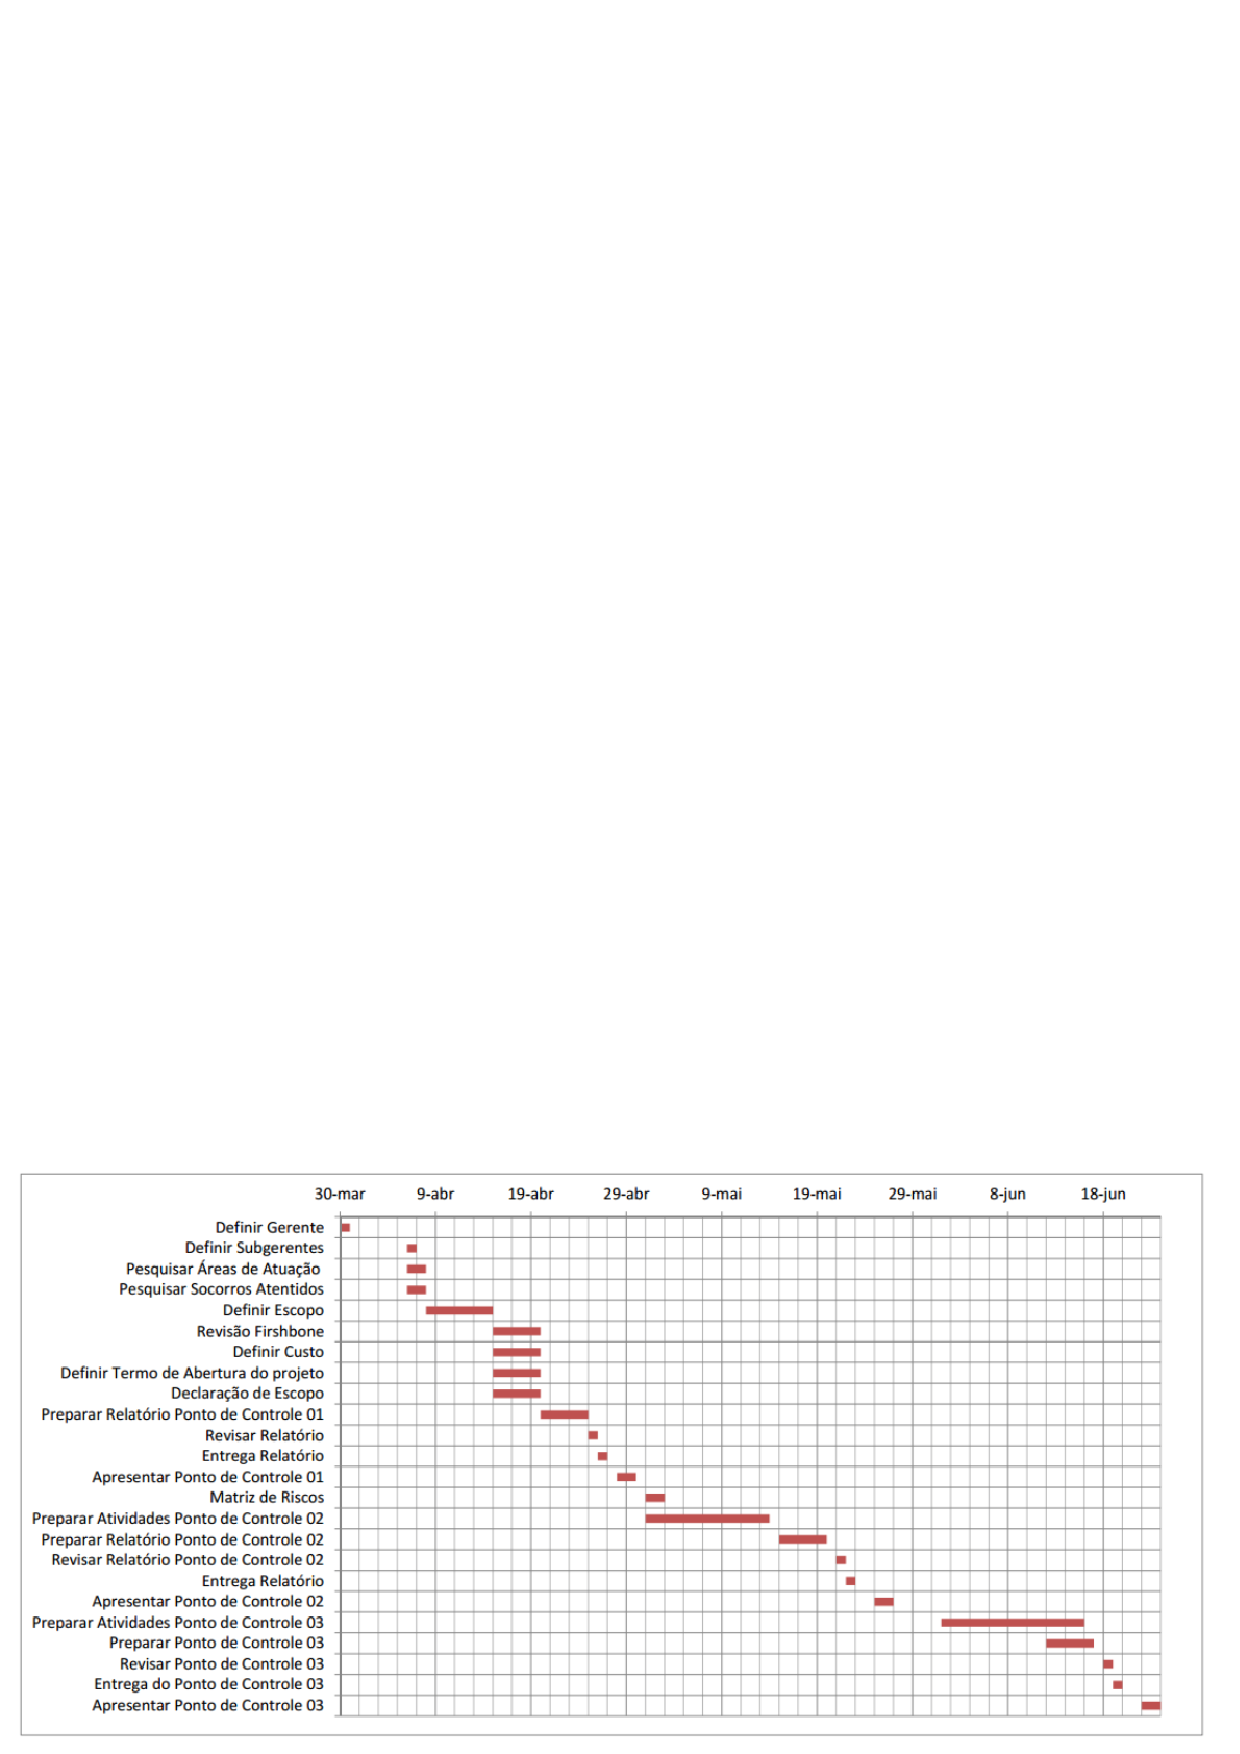
\includegraphics[keepaspectratio=true,scale=0.4,angle=90]{figuras/gantt.png}
	\caption{Gráfico de Gantt}
\end{figure}
